\clearpage
\section{Evaluation}
For evaluation, we measure time, error rate and the consistency of each trials.
If time is fast, it means the system is easy to operate.
If the average error is low, it means the system is accurate.
If time and average error does not change for every trial, it means the system is stable.
\par
We only evaluate about 'drawing' function because 'drawing' function is the most essential function of the system.
We evaluate this system using three tasks. Fig. \ref{task} shows three examples.
The flow of the evaluation is as follows. At first, there is a white canvas and pointer.
When the tester press 'r', it shows the sample to trace and starts timer.
User starts drawing and when he finish drawing, the tester press 'q' and timer ends.
The user do same task three times.
Time is measured by this timer. The average error is measured by the difference between the example and what he draw. The consistency is measured by the standard deviation of time and average error.
\par
To compare the results, we also tested the mouse as the input device. When we point a point in the canvas using a mouse, the pointer moves. When we drag with left click, it draws a line.\par
We used user as both of our team member.
\subsection{The average error measurement}
\subsubsection{Points}
We measure the distance between what the user draw and the nearest point of the sample.
To make the measurement easy, we divide the canvas into 4 section.
If a point the user draw is on upper left, we compare the distance with upper left point of the sample. Same as upper right, lower left and lower right.
\subsubsection{Circle}
Circle is the points which distance from the center point are radius.
We know the center point and the radius of the sample circle.
Thus we measure the absolute difference between radius and the actual difference from the center point for each points. Then we average them.
\subsubsection{Line}
We measure the distance between the actual line and sample line by comparing only 20 points of the lines. We equally sample 20 points in the lines along the vertical axis. And from the most highest points to the most lowest Points, we measure the difference of them.
Fig.\ref{linem} shows the example. Blue line is a sample line and red line is user's line. The points are sample points. Each points are measured with the points which are connected by the black line.
\begin{figure}
\begin{tabular}{|c|c|c|}
 Points & circle & line \\ \hline
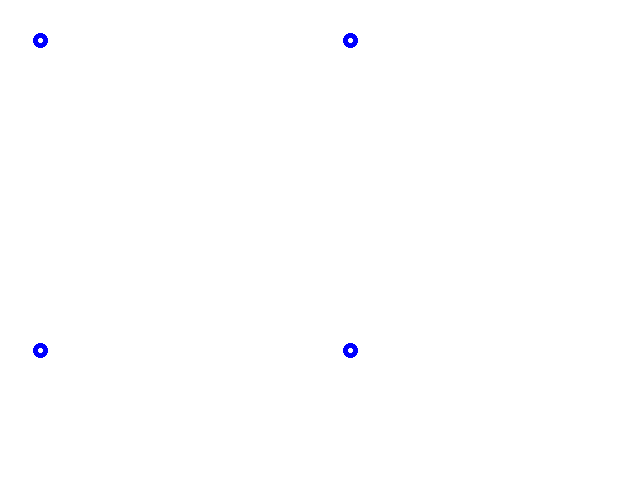
\includegraphics[width=4cm]{fig_exp/points.png} &
 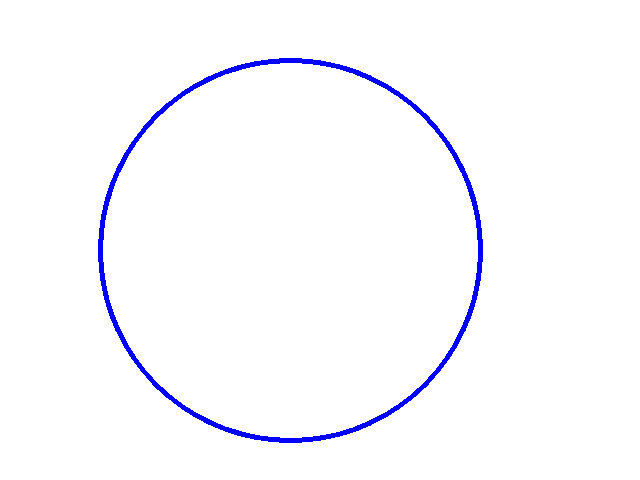
\includegraphics[width=4cm]{fig_exp/circle.png} &
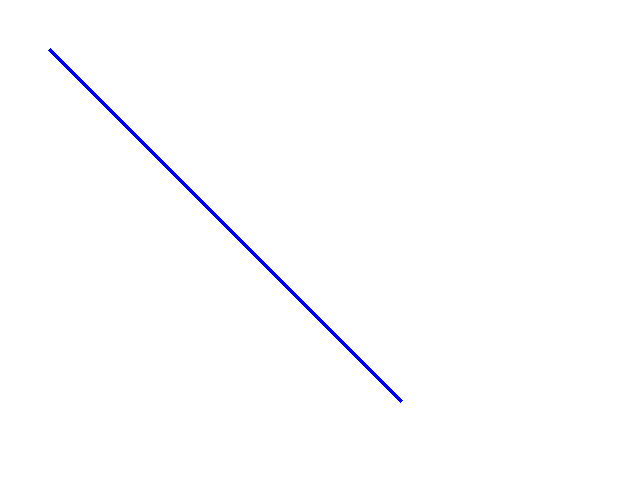
\includegraphics[width=4cm]{fig_exp/line.png}
\end{tabular}

 \caption{Three tasks}
 \label{task}
\end{figure}

\begin{figure}[htbp]
 \centering
 \begin{tikzpicture}
 \draw (0, 0) -- ++(30:4);
 \draw[red] (0, -1) -- ++ (-30:1.5);
 \draw[red] (0, -1) + (-30:3.5) -- ++(-30:6);
 \draw[dashed,fill] (0, 0) circle (2pt) -- (0, -1);
 \draw[dashed,fill] (0, 0) + (30:1) circle (2pt) -- ($(0, -1) + (-30:1)$);
 \draw[dashed,fill] (0, 0) + (30:2) circle (2pt) -- ($(0, -1) + (-30:4)$);
 \draw[dashed,fill] (0, 0) + (30:3) circle (2pt) -- ($(0, -1) + (-30:5)$);
 \draw[dashed,fill] (0, 0) + (30:4) circle (2pt) -- ($(0, -1) + (-30:6)$);
 \draw[fill=red] (0, -1)           circle (2pt);
 \draw[fill=red] (0, -1) + (-30:1) circle (2pt);
 \draw[fill=red] (0, -1) + (-30:4) circle (2pt);
 \draw[fill=red] (0, -1) + (-30:5) circle (2pt);
 \draw[fill=red] (0, -1) + (-30:6) circle (2pt);

\end{tikzpicture}

 \caption{Line error measurement}
 \label{linem}
\end{figure}


\subsection{Results}
Table \ref{tb:p2} shows the measurement results of the points task. Table \ref{tb:c1} and Table \ref{tb:c2} show the results of the circle task and the actual canvas image. Table \ref{tb:l1} and Table \ref{tb:l2} show the results of the line task and the actual canvas image. Table \ref{tb:exp} shows the standard deviation of them. In all tasks, mouse device results are better than our input device. Among three tasks, for our device performance is better in circle task. We can see the time deviation is better than the error deviation.

\begin{table}[htbp]
 \centering
 \caption{The result of the user study (points)}
 \label{tb:p2}
 \begin{tabular}{llrrr}
 \toprule
 User & Device & Trial & Time[sec] & Error [pixels] \\
 \midrule
A	&	VI	&	1	&	13.32	&	68.558	\\
A	&	VI	&	2	&	14.522	&	88.314	\\
A	&	VI	&	3	&	15.282	&	68.406	\\
B	&	VI	&	1	&	17.87	&	72.838	\\
B	&	VI	&	2	&	12.132	&	68.172	\\
B	&	VI	&	3	&	6.599	&	71.913	\\
C	&	VI	&	1	&	13.127	&	74.432	\\
C	&	VI	&	2	&	14.004	&	51.564	\\
C	&	VI	&	3	&	13.183	&	67.076	\\
A	&	VI2	&	1	&	11.856	&	63.8	\\
A	&	VI2	&	2	&	12.086	&	58.081	\\
A	&	VI2	&	3	&	18.693	&	89.614	\\
B	&	VI2	&	1	&	10.93	&	88.821	\\
B	&	VI2	&	2	&	13.809	&	104.269	\\
B	&	VI2	&	3	&	8.009	&	67.539	\\
C	&	VI2	&	1	&	18.943	&	31.226	\\
C	&	VI2	&	2	&	17.128	&	66.85	\\
C	&	VI2	&	3	&	16.892	&	87.412	\\
A	&	Mouse	&	1	&	6.716	&	4.125	\\
A	&	Mouse	&	2	&	7.444	&	10.296	\\
A	&	Mouse	&	3	&	7	&	4.634	\\
B	&	Mouse	&	1	&	8.113	&	4.746	\\
B	&	Mouse	&	2	&	6.293	&	8.115	\\
B	&	Mouse	&	3	&	6.428	&	7.388	\\
C	&	Mouse	&	1	&	5.4	&	4.989	\\
C	&	Mouse	&	2	&	5.481	&	4.768	\\
C	&	Mouse	&	3	&	5.199	&	6.603	\\
 \bottomrule
\end{tabular}

\end{table}


\begin{table}[htbp]
 \centering
 \caption{The result of the user study (circle)}
 \label{tb:c1}
 \begin{tabular}{lccc}
\toprule
 & Trial 1 & Trial 2 & Trial 3\\
\midrule
 User A (VI)&
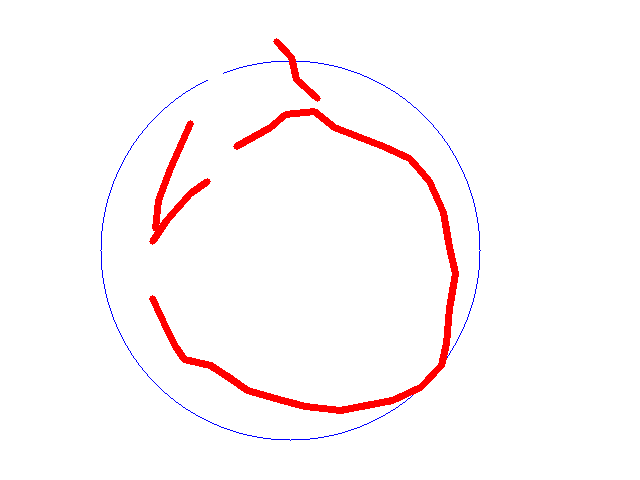
\includegraphics[width=3cm]{fig_exp/circle_Ayaka_test3_0.png} &
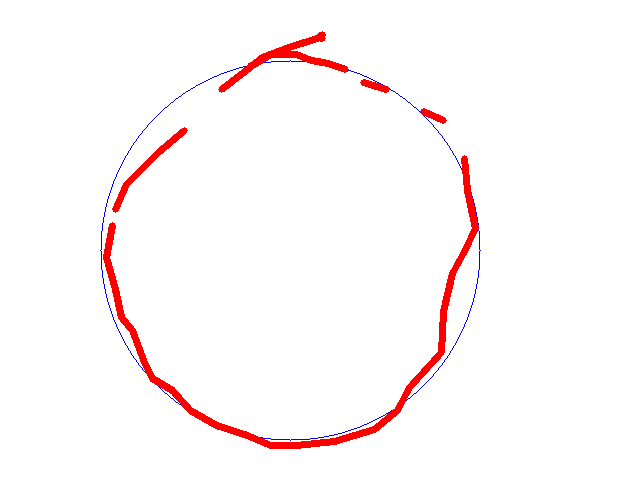
\includegraphics[width=3cm]{fig_exp/circle_Ayaka_test3_1.png} &
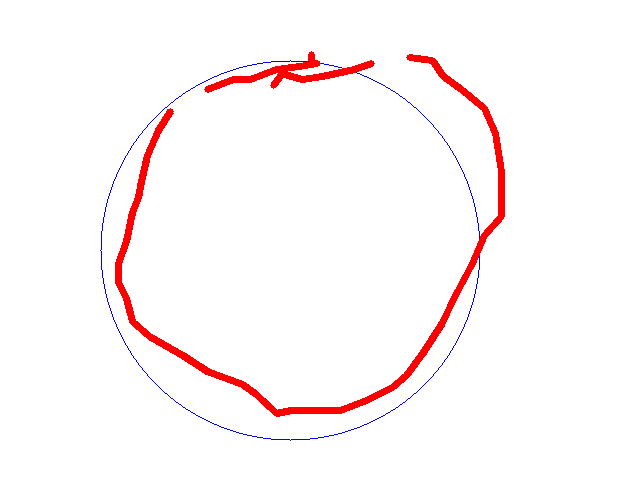
\includegraphics[width=3cm]{fig_exp/circle_Ayaka_test3_2.png} \\
\midrule
 User B (VI)&
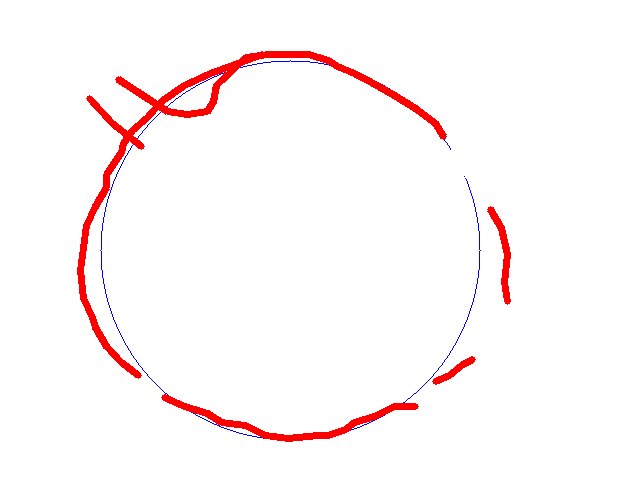
\includegraphics[width=3cm]{fig_exp/circle_Angus_test3_0.png} &
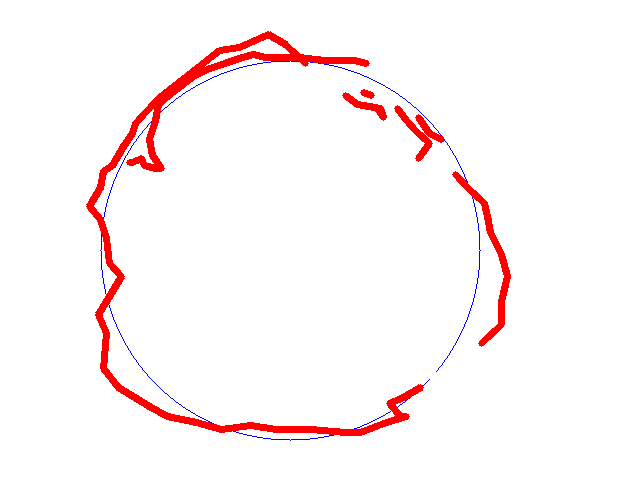
\includegraphics[width=3cm]{fig_exp/circle_Angus_test3_1.png} &
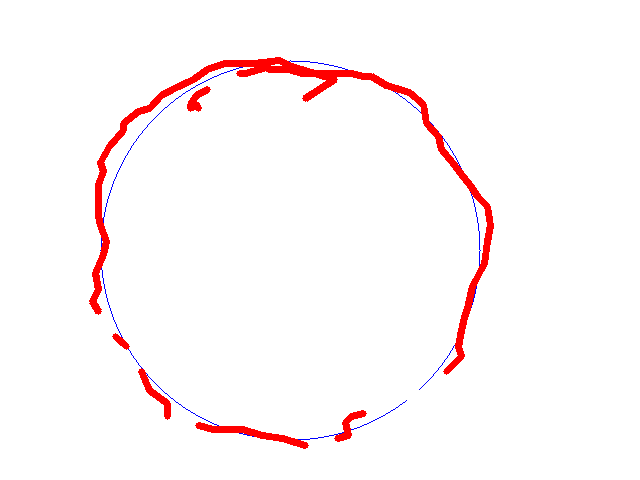
\includegraphics[width=3cm]{fig_exp/circle_Angus_test3_2.png} \\
\midrule
 User A (Mouse)&
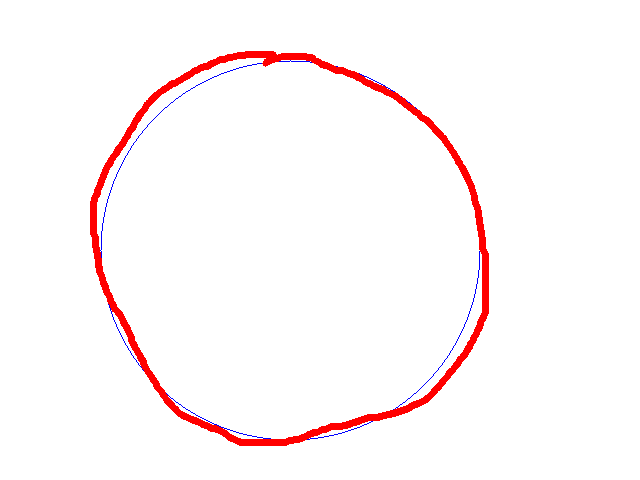
\includegraphics[width=3cm]{fig_exp/circle_Ayaka_test3_0_m.png} &
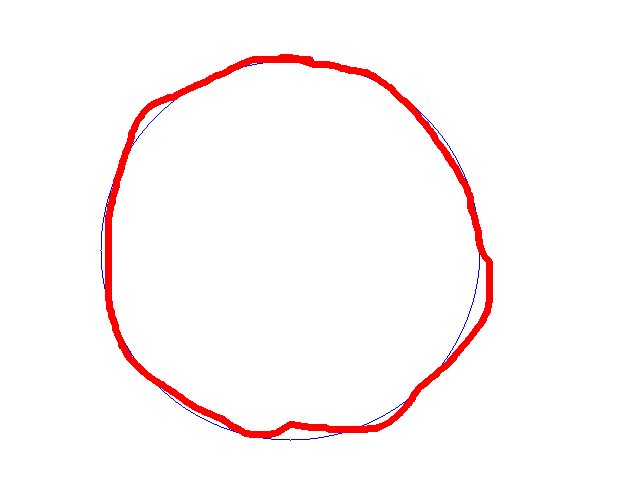
\includegraphics[width=3cm]{fig_exp/circle_Ayaka_test3_1_m.png} &
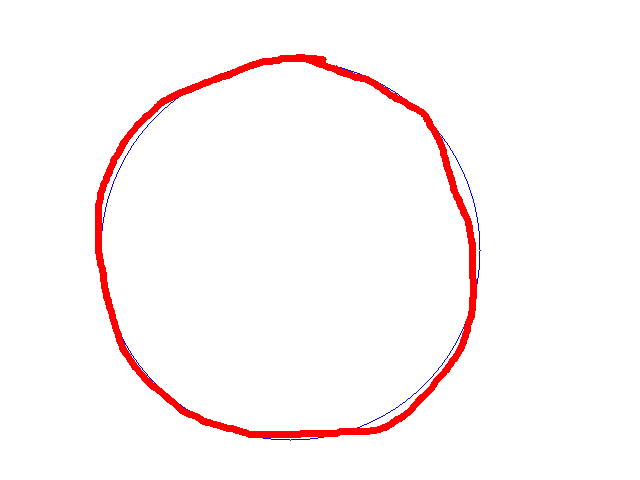
\includegraphics[width=3cm]{fig_exp/circle_Ayaka_test3_2_m.png} \\
\midrule
 User B (Mouse)&
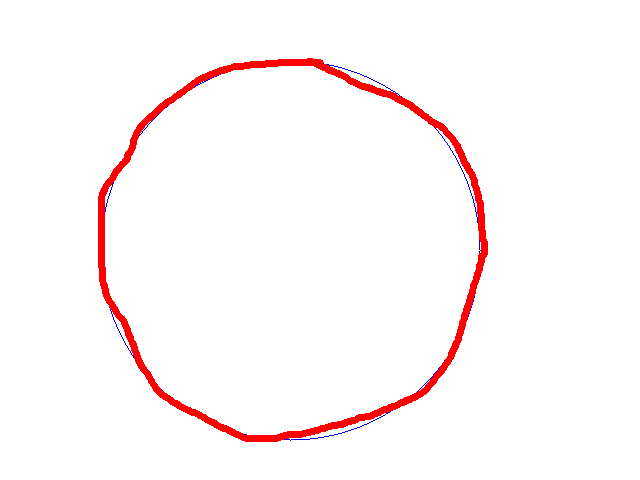
\includegraphics[width=3cm]{fig_exp/circle_Angus_test3_0_m.png} &
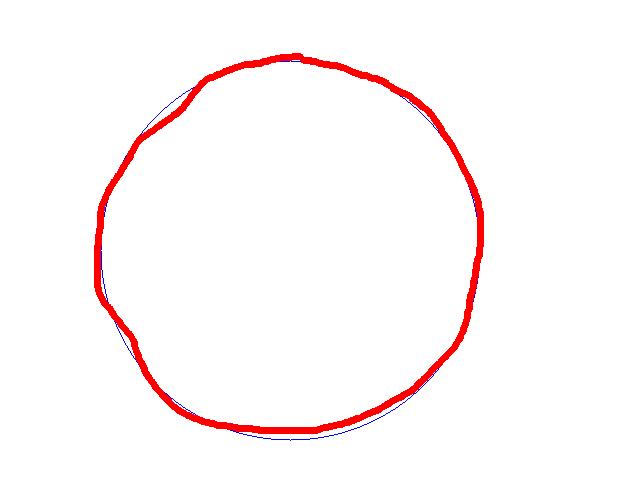
\includegraphics[width=3cm]{fig_exp/circle_Angus_test3_1_m.png} &
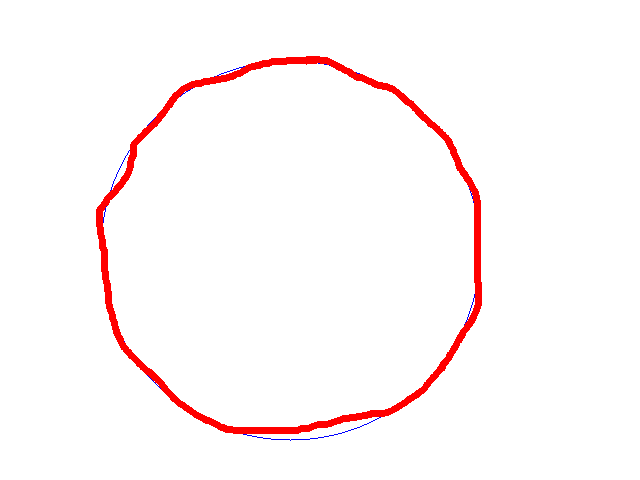
\includegraphics[width=3cm]{fig_exp/circle_Angus_test3_2_m.png} \\
\bottomrule
\end{tabular}


\end{table}



\begin{table}[htbp]
 \centering
 \caption{The result of the user study (circle)}
 \label{tb:c2}
 \begin{tabular}{llrrr}
 \toprule
 User & Device & Trial & Time[sec] & Error [pixels] \\
 \midrule
A	&	VI	&	1	&	14.507	&	12.745	\\
A	&	VI	&	2	&	17.756	&	18.283	\\
A	&	VI	&	3	&	20.314	&	17.653	\\
B	&	VI	&	1	&	8.131	&	24.242	\\
B	&	VI	&	2	&	7.84	&	14.619	\\
B	&	VI	&	3	&	7.962	&	13.559	\\
C	&	VI	&	1	&	8.433	&	46.652	\\
C	&	VI	&	2	&	10.818	&	17.856	\\
C	&	VI	&	3	&	11.376	&	10.398	\\
A	&	VI2	&	1	&	20.229	&	6.966	\\
A	&	VI2	&	2	&	17.148	&	9.991	\\
A	&	VI2	&	3	&	17.836	&	7.156	\\
B	&	VI2	&	1	&	10.819	&	12.892	\\
B	&	VI2	&	2	&	11.19	&	13.977	\\
B	&	VI2	&	3	&	12.79	&	17.879	\\
C	&	VI2	&	1	&	10.963	&	12.154	\\
C	&	VI2	&	2	&	11.597	&	7.066	\\
C	&	VI2	&	3	&	12.712	&	8.156	\\
A	&	Mouse	&	1	&	8.187	&	8.815	\\
A	&	Mouse	&	2	&	10.502	&	4.736	\\
A	&	Mouse	&	3	&	9.929	&	5.995	\\
B	&	Mouse	&	1	&	8.801	&	4.548	\\
B	&	Mouse	&	2	&	7.999	&	4.067	\\
B	&	Mouse	&	3	&	8.039	&	4.741	\\
C	&	Mouse	&	1	&	7.474	&	6.215	\\
C	&	Mouse	&	2	&	7.187	&	6.929	\\
C	&	Mouse	&	3	&	7.519	&	5.348	\\
 \bottomrule
\end{tabular}

\end{table}

\begin{table}[htbp]
 \centering
 \caption{The result of the user study (line)}
 \label{tb:l1}
 \begin{tabular}{lccc}
\toprule
 & Trial 1 & Trial 2 & Trial 3\\
\midrule
 User A (VI)&
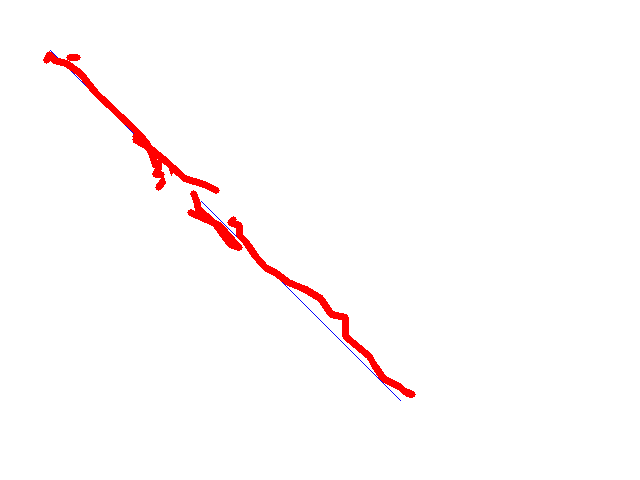
\includegraphics[width=3cm]{fig_exp/line_Ayaka_test3_0.png} &
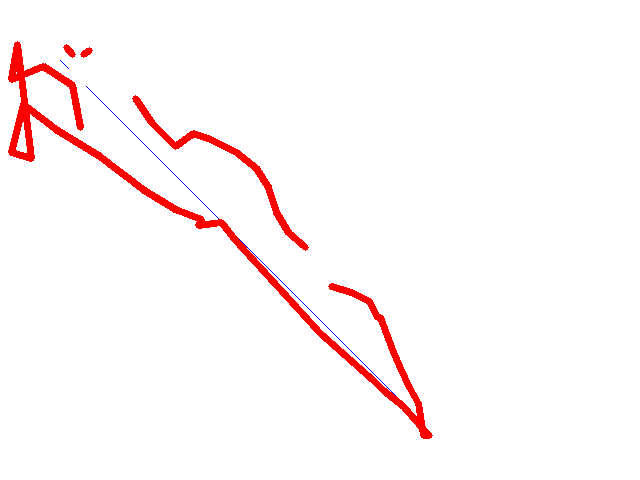
\includegraphics[width=3cm]{fig_exp/line_Ayaka_test3_1.png} &
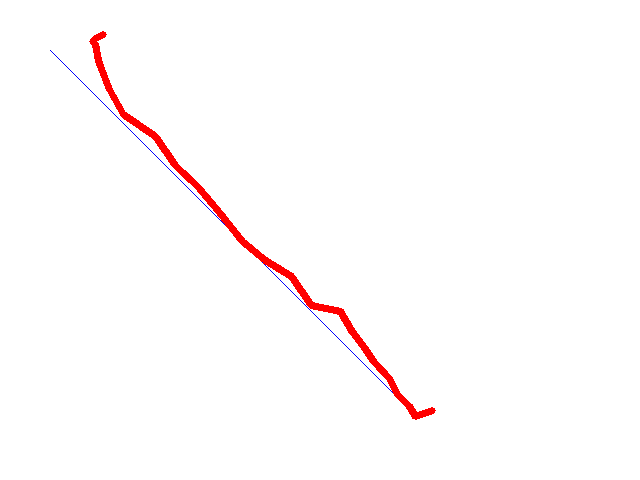
\includegraphics[width=3cm]{fig_exp/line_Ayaka_test3_2.png} \\
\midrule
 User B (VI)&
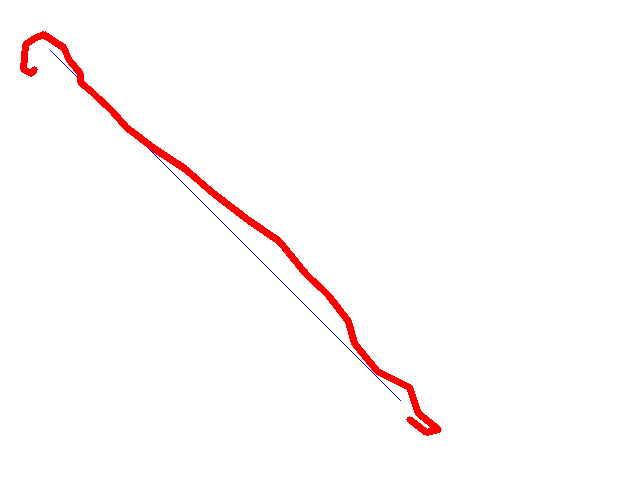
\includegraphics[width=3cm]{fig_exp/line_Angus_test3_0.png} &
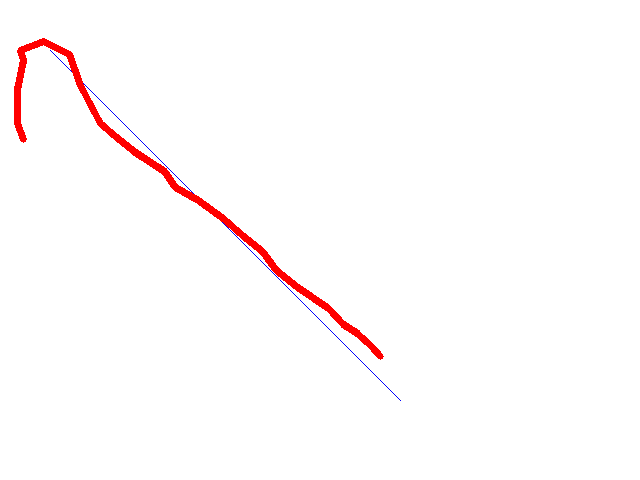
\includegraphics[width=3cm]{fig_exp/line_Angus_test3_1.png} &
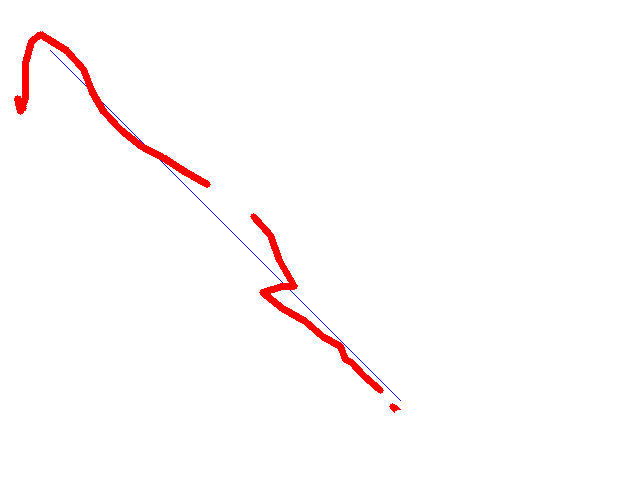
\includegraphics[width=3cm]{fig_exp/line_Angus_test3_2.png} \\
\midrule
 User A (Mouse)&
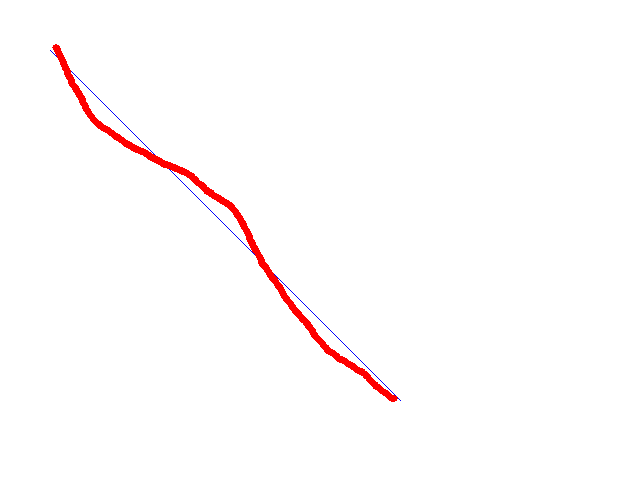
\includegraphics[width=3cm]{fig_exp/line_Ayaka_test3_0_m.png} &
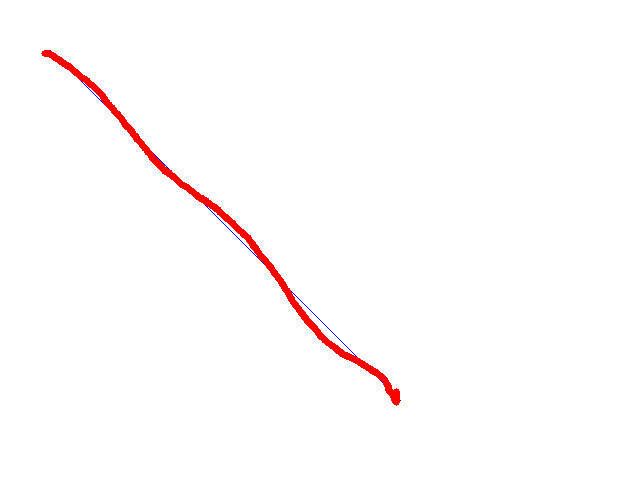
\includegraphics[width=3cm]{fig_exp/line_Ayaka_test3_1_m.png} &
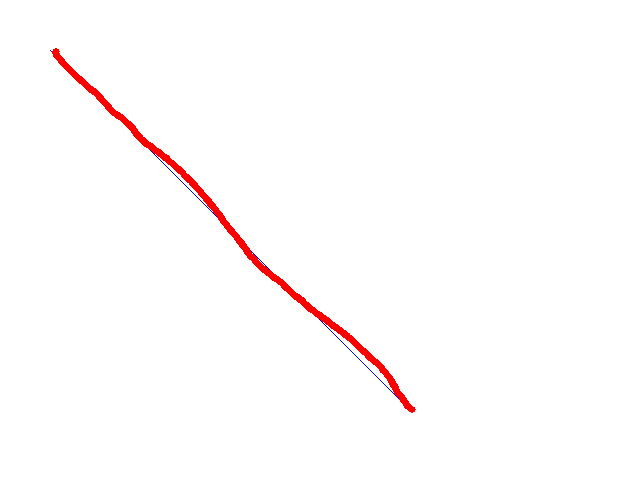
\includegraphics[width=3cm]{fig_exp/line_Ayaka_test3_2_m.png} \\
\midrule
 User B (Mouse)&
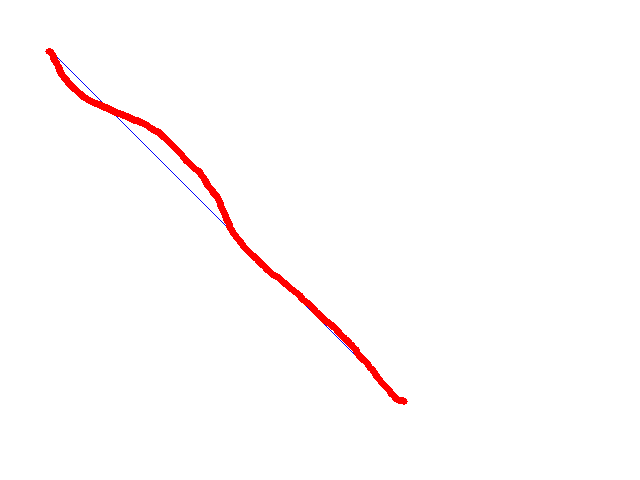
\includegraphics[width=3cm]{fig_exp/line_Angus_test3_0_m.png} &
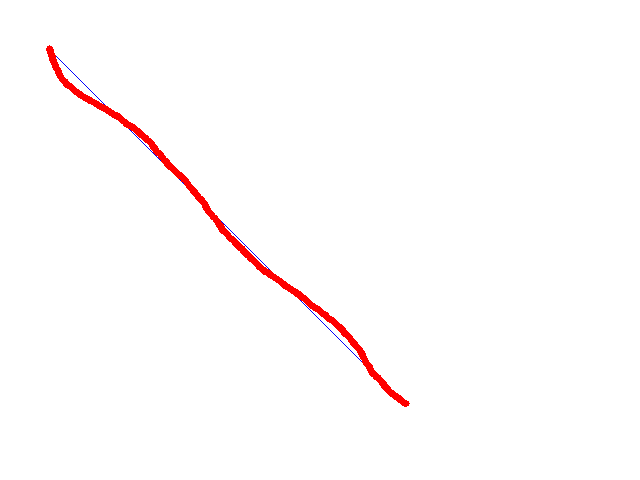
\includegraphics[width=3cm]{fig_exp/line_Angus_test3_1_m.png} &
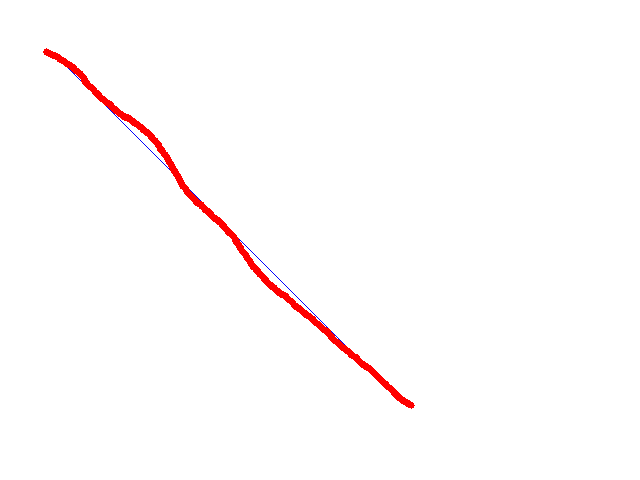
\includegraphics[width=3cm]{fig_exp/line_Angus_test3_2_m.png} \\
\bottomrule
\end{tabular}

\end{table}


\begin{table}[htbp]
 \centering
 \caption{The result of the user study (line)}
 \begin{tabular}{llrrr}
 \toprule
 User & Device & Trial & Time[sec] & Error Pixels \\
 \midrule
 A	& VI	  & 1	& 20.16	& 22.25 \\
 A	& VI	  & 2	& 14.75	& 76.46 \\
 A	& VI	  & 3	& 5.73	& 25.77 \\
 B	& VI	  & 1	& 7.76	& 39.92 \\
 B	& VI	  & 2	& 8.03	& 88.50 \\
 B	& VI	  & 3	& 10.03	& 58.27 \\
 A	& Mouse	& 1	& 4.07	& 13.87 \\
 A	& Mouse	& 2	& 5.19	& 6.53 \\
 A	& Mouse	& 3	& 4.07	& 8.01 \\
 B	& Mouse	& 1	& 3.98	& 8.99 \\
 B	& Mouse	& 2	& 4.83	& 7.24 \\
 B	& Mouse	& 3	& 4.61	& 7.71 \\
 \bottomrule
\end{tabular}

 \label{tb:l2}
\end{table}




\begin{table}[htbp]
 \centering
 \caption{Standard Deviation of User study}
 \label{tb:exp}
 \begin{tabular}{lllrr}
 \toprule
 Task & User & Device & StdDev of Time & StdDev of Error \\
 \midrule
 Points	& A	& VI	  & 2.20	& 9.87 \\
 Points	& B	& VI	  & 1.37	& 10.06 \\
 Points	& A	& Mouse	& 0.83	& 1.29 \\
 Points	& B	& Mouse	& 0.46	& 0.31 \\
 Circle	& A	& VI	  & 0.28	& 11.75 \\
 Circle	& B	& VI	  & 1.88	& 2.23 \\
 Circle	& A	& Mouse	& 0.07	& 0.80 \\
 Circle	& B	& Mouse	& 0.25	& 0.26 \\
 Line	  & A	& VI	  & 5.95	& 24.77 \\
 Line	  & B	& VI	  & 1.01	& 20.03 \\
 Line	  & A	& Mouse	& 0.53	& 3.17 \\
 Line	  & B	& Mouse	& 0.36	& 0.74 \\
 \bottomrule
\end{tabular}

\end{table}
